\chapter{\IfLanguageName{dutch}{Stand van zaken}{State of the art}}%
\label{ch:stand-van-zaken}

% Tip: Begin elk hoofdstuk met een paragraaf inleiding die beschrijft hoe
% dit hoofdstuk past binnen het geheel van de bachelorproef. Geef in het
% bijzonder aan wat de link is met het vorige en volgende hoofdstuk.

% Pas na deze inleidende paragraaf komt de eerste sectiehoofding.

Zoals in hoofdstuk \ref{ch:inleiding} werd vermeld, wordt er een oplossing gezocht voor het slim aansturen van bepaalde bedrijfsprocessen van het bedrijf Carwash Clean Car. Voordat er oplossingen kunnen worden besproken, is het belangrijk dat er een grondige voorkennis wordt opgedaan over het onderwerp. Deze literatuurstudie zal daarbij helpen. Om tot een geschikte oplossing te komen, is de literatuurstudie opgedeeld in 3 delen. In afbeelding \ref{fig:voorlopige-proefopstelling} wordt de voorlopige versie van de proefopstelling weergegeven, zodat een idee kan gevormd worden over hoe alles zal samenwerken.

\begin{figure}[htbp]
    \centering
    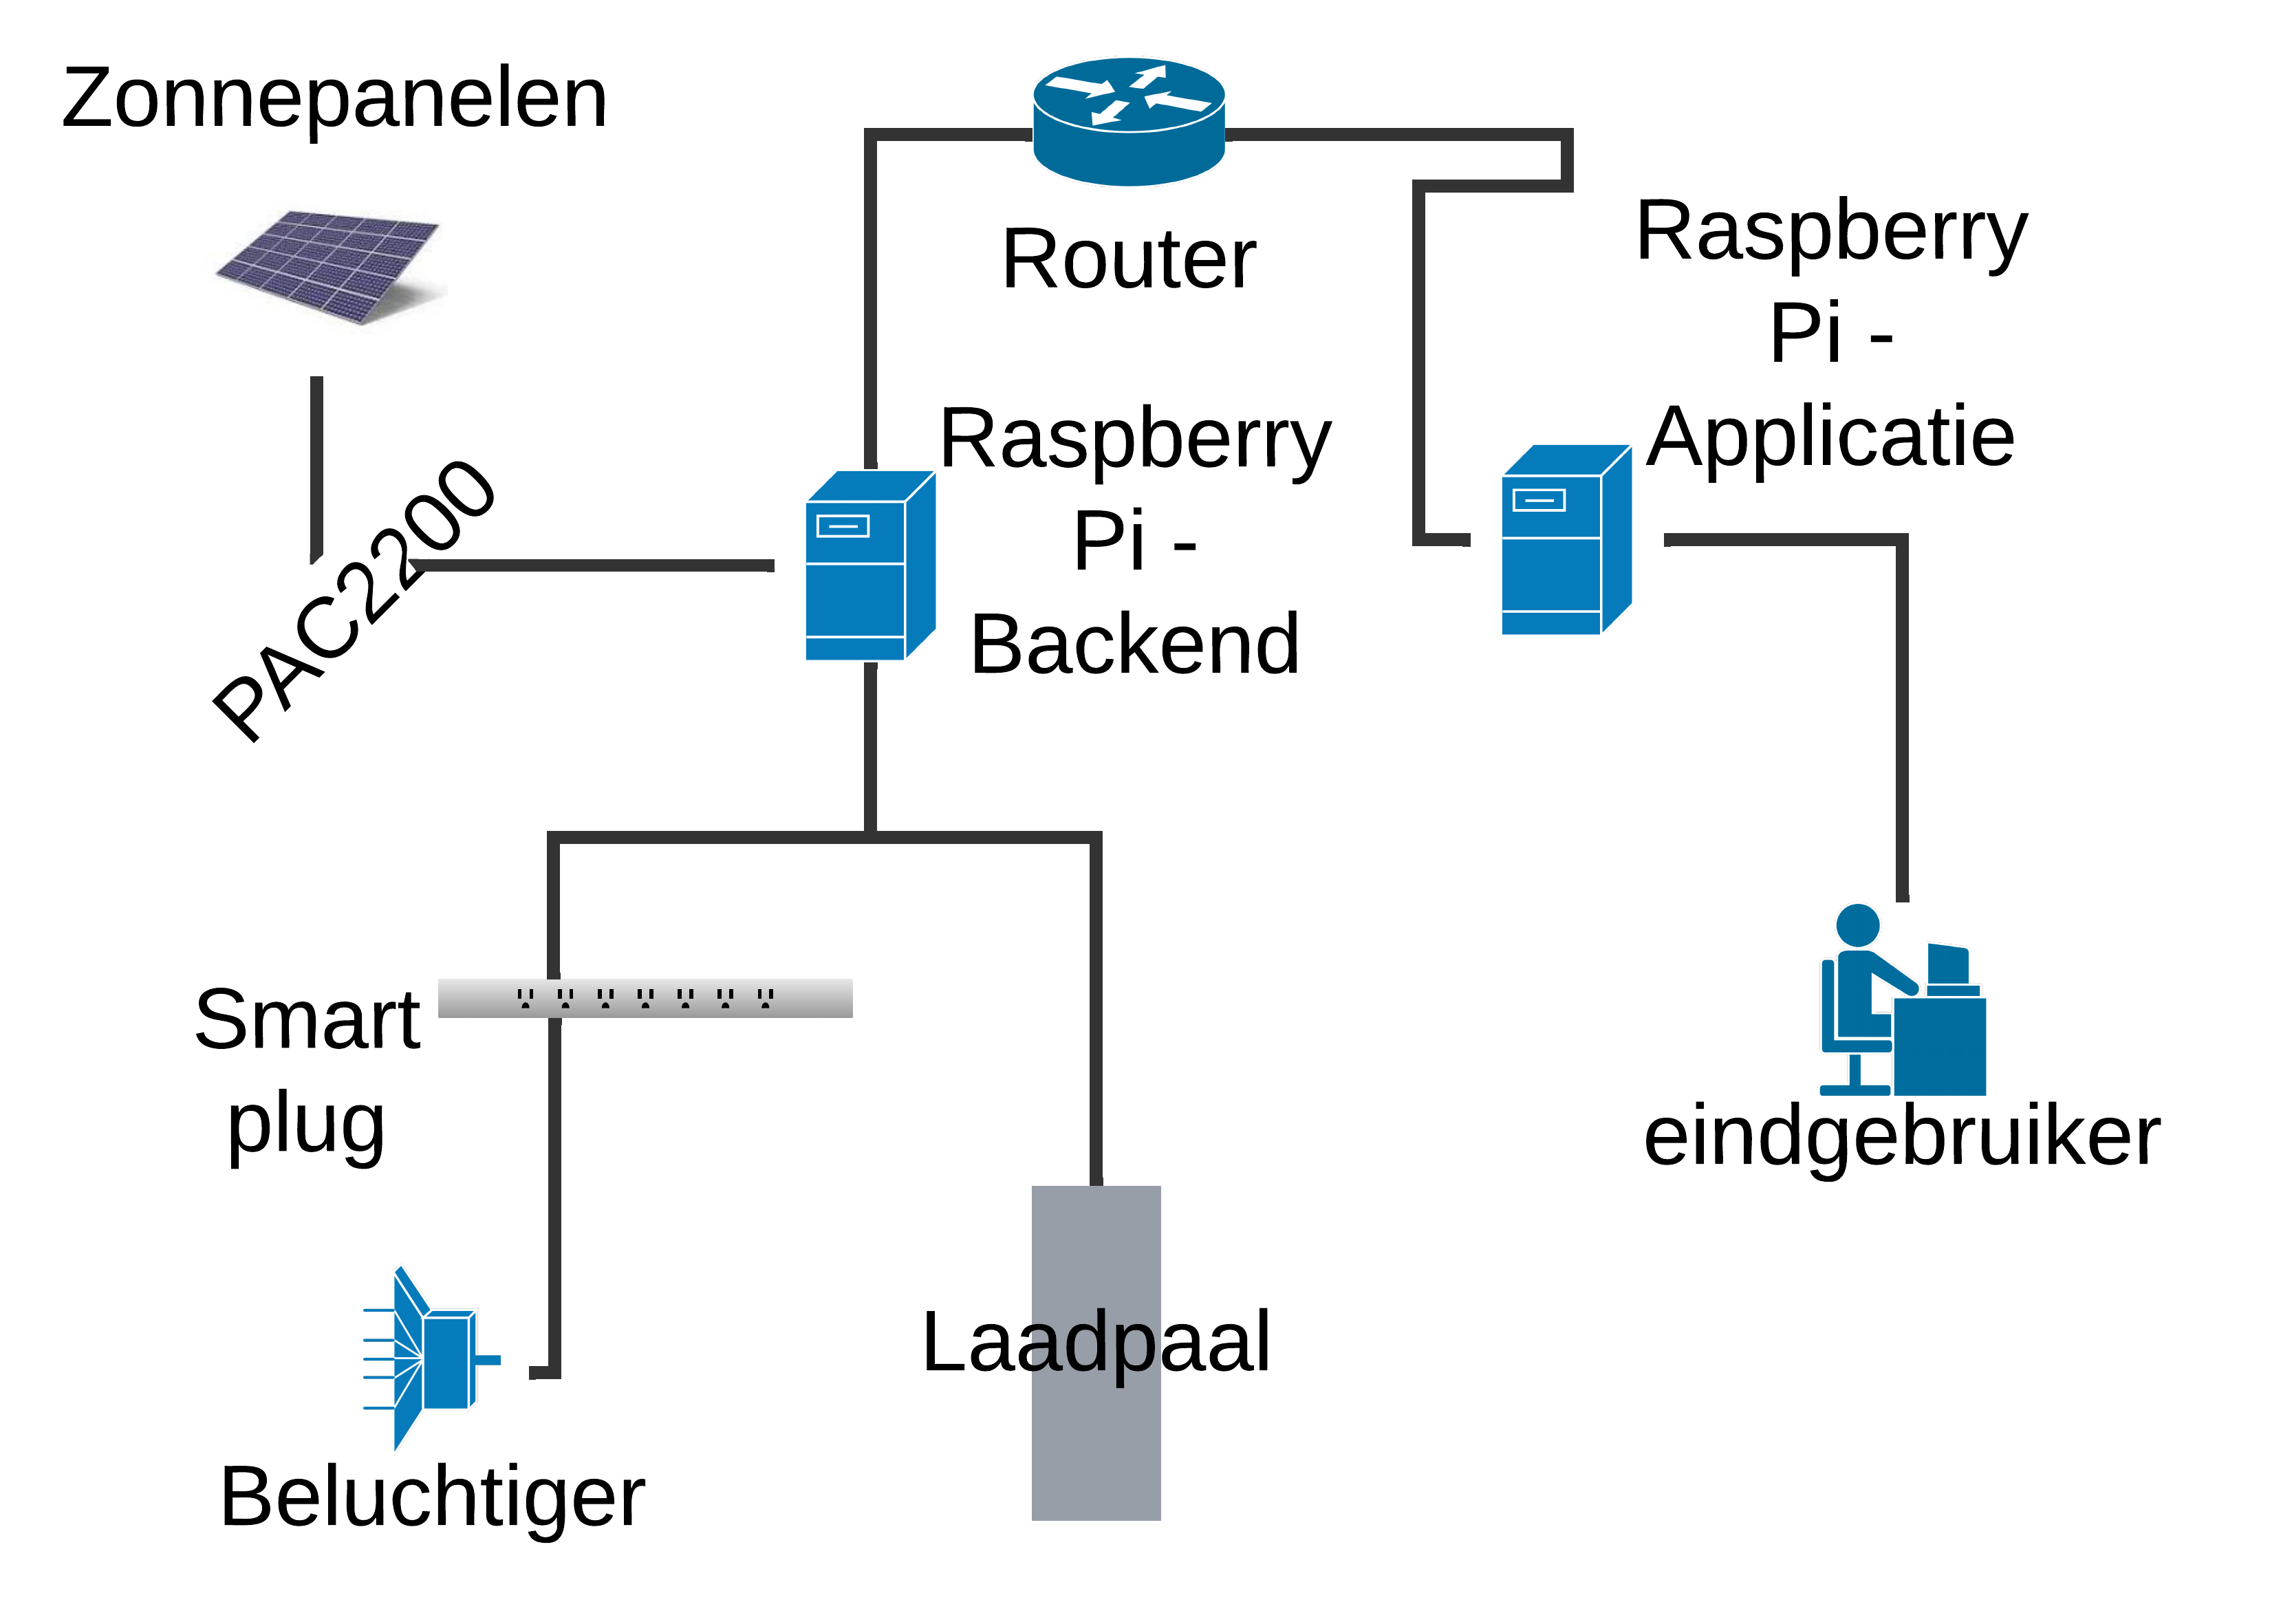
\includegraphics[width=20em]{./graphics/voorlopige-proefopstelling.png}
    \caption{Voorlopige ilustratie van de proefopstelling}
     \label{fig:voorlopige-proefopstelling}
\end{figure}

\pagebreak

\section{Hoe kwam carwash Clean Car op dit idee?}
\label{sec:stand-van-zaken-idee}

Carwash Clean Car heeft in 2013 zonnepanelen geplaatst, omdat de eigenaar toen al merkte dat als alle apparatuur van de carwash samen moest aanstaan, deze de energiefactuur te duur maakte. Hierbij werd ook rekening gehouden met de plannen om een extra self carwash met 5 wasboxen te plaatsen op het domein. Toen deze self carwash geplaatst was in 2015, merkte de eigenaar toch op dat er niet altijd genoeg zonne-energie werd geproduceerd door de zonnepanelen, om de elektriciteit-intensieve bedrijfsprocessen aan te sturen. Er werd dus nog altijd veel energie aangekocht. Bovenop het tekort aan zonne-energie, werden de energieprijzen steeds maar duurder.\\

Een paar jaar later besliste het bedrijf om hun bedrijfswagen op fossiele brandstof te vervangen door een elektrische wagen. Hierdoor werd er ook een laadpaal van Alfen geplaatst die slim aan te sturen is. Zo kwam carwash Clean Car op het idee om alle niet-dringende bedrijfsprocessen slim aan te sturen door middel van een custom webapplicatie en daarbij het laden van die wagen op een slimme manier te laten gebeuren.

\section{Energieverbruikers van carwash Clean Car}
\label{sec:stand-van-zaken-energieverbruikers}

Aangezien deze casus zich richt op een carwash, is 1 van de belangrijkste energieverbruikers de machines en infrastructuur die gebruikt wordt om de tunnel van de carwash aan te sturen. De tunnel kan opgedeeld worden in 2 delen, het eerste deel dient voor het wassen van de auto’s, wat gemiddeld 5 kilowatt verbruikt per auto. Het tweede deel van de tunnel zorgt voor het drogen van de auto’s, dit verbruikt gemiddeld 50 kilowatt.\\

Naast deze tunnel is er ook nog de self carwash, die op het domein gevestigd is. De infrastructuur van deze self carwash hoort dan ook bij de belangrijkste energieverbruikers van het bedrijf. De selfcarwash bestaat uit 5 wasboxen. Als 1 box in gebruik is, wordt 1 pomp geactiveerd en wordt er 2 kilowatt verbruikt. Voor de 5 wasboxen tegelijk, wordt het verbruik dus 10 kilowatt.\\

Na de 2 belangrijkste energieverbruikers zijn er ook verschillende niet-dringende energieverbruikers die toch wel belangrijk zijn voor de eigenaars, zo staat er een laadpaal geïnstalleerd, deze laadpaal wordt gebruikt voor het opladen van elektrische voertuigen, zodat deze kunnen gebruikt worden wanneer het nodig is. Het laadvermogen van de laadpaal kan zelf ingesteld worden tot en met 11 kilowatt.\\

De tweede niet-dringende energieverbruiker is het beluchtingssysteem van het water, dit systeem is nodig om te voorkomen dat er algen ontstaan in het zelf gerecycleerde water in de waterputten. Het beluchtingssysteem heeft een vermogen van 3 kilowatt. Deze 3 kilowatt fluctueert niet, wat betekent dat het beluchtingssysteem continu 3 kilowatt verbruikt wanneer deze ingeschakeld wordt. Het systeem is niet continu ingeschakeld om schuimvorming te voorkomen.\\

De laatste energieverbruiker die besproken wordt is de industriële droogkast, deze droogkast wordt gebruikt voor het drogen van de werkkledij en de microvezeldoeken die gebruikt worden bij dieptereinigingen. De reden dat deze droogkast besproken wordt is omdat deze al verouderd en energie-intensief is. De droogkast is tot nu toe het niet-dringende bedrijfsproces met het hoogste verbruik. Het energieverbruik is namelijk 14 kilowatt.\\

De tunnel en self carwash worden in de proefopstelling niet aangesproken, omdat deze niet zomaar uitgeschakeld mogen worden. De industriële droogkast wordt na deze bachelorproef pas toegevoegd aan de proefopstelling, de oorzaak hiervan is dat de componenten om de droogkast slim aan te sturen nog besteld moeten worden. Al de rest van de besproken niet-dringende bedrijfsprocessen zullen wel al geïntegreerd worden met webapplicatie. 

\section{Peak shaving}
\label{sec:stand-van-zaken-peak-shaving}

Het eerste concept dat besproken wordt is peak shaving. De bedoeling van dit concept is om pieken in de aankoop van energie af te vlakken, dit kan gebeuren door bepaalde bedrijfsprocessen te verplaatsen naar momenten waar er minder energie verbruikt wordt of er te veel energie geïnjecteerd wordt op het energienet. Deze methode zorgt voor een meer gelijkvormige verdeling van het energieverbruik.\\

Er zijn verschillende methoden om peak shaving te bereiken, “1 methode van peak shaving is het gebruik van een energieopslagsysteem" \autocite{UDDIN2018}. Om deze methode te gebruiken zijn er batterijen nodig die energie kunnen opslaan, deze batterijen stellen het energieopslagsysteem voor. “Bij deze methode wordt peak shaving bereikt door de batterijen op te laden wanneer de vraag naar elektriciteit laag is, ook wel een dalperiode genoemd. Deze batterijen kunnen dan ontladen worden als de vraag naar elektriciteit hoog is. Deze methode kan economische voordelen opleveren voor het bedrijf, omdat tijdens de hoge vraag naar elektriciteit de batterijen gebruikt kunnen worden" \autocite{UDDIN2018}.

\section{Bidirectioneel laden van batterijen}
\label{sec:stand-van-zaken-bidirectioneel-laden}

1 van de concepten die aan het opkomen is bij laadpalen is bidirectioneel laden. Dit betekent dat, als een auto opgeladen wordt, deze auto batterij gebruikt kan worden om energie op te slaan voor later gebruik. Wat betekent dat de wagen ook energie kan teruggeven via de laadpaal. Dit zou handig zijn om niet-dringende bedrijfsprocessen aan te sturen als er energie aangekocht wordt. Dit concept kan ook toegepast worden op reserve batterijen die geïnstalleerd worden voor als de elektriciteit wegvalt.\\

Voor het gebruik van bidirectioneel laden van een auto is er een elektrische auto en een laadpaal nodig die dit ondersteunt. Er zijn al verschillende bedrijven die dit concept toepassen op hun wagens. Gelukkig heeft de eigenaar van het bedrijf hier rekening mee gehouden bij de aankoop van de ID. Buzz van Volkswagen. De huidige laadpaal daarentegen heeft deze functionaliteit nog niet, waardoor deze nog niet benut kan worden.\\

Het verschil tussen een laadpaal die de functie van bidirectioneel laden niet heeft en een laadpaal die de functie wel heeft, heeft te maken met het type van elektrische stroom, zo bestaan er twee types van elektrische stroom namelijk wisselstroom (AC) en gelijkstroom (DC). Zo kan bidirectioneel laden voor 2 toepassingen worden gebruikt, namelijk Vehicle-to-Grid (V2G) en Vehicle-to-Home (V2H), “vehicle-to-grid is bedoeld voor het verkopen van opgeslagen energie aan het energienet. Terwijl vehicle-to-home daarentegen bedoeld is om de opgeslagen energie later zelf thuis te gebruiken” \autocite{LAZZERONI2019}.\\

Het interessantste voor het bedrijf is de vehicle-to-home oplossing, omdat als de elektriciteit wegvalt, er kan overgeschakeld worden op de batterij van de ID. buzz of reserve batterijen. Het voordeel hiervan is dat de elektriciteit niet moet wegvallen om de batterij van de ID. buzz te gebruiken, waardoor als er enkel energie aangekocht wordt er andere niet-dringende bedrijfsprocessen hiermee verder kunnen worden aangestuurd. De reden dat er niet voor de vehicle-to-grid oplossing gekozen wordt is omdat het bedrijf minder elektriciteit wil injecteren op het energienet, aangezien hier bijna niets aan verdiend wordt. Het is immers juist de bedoeling van vehicle-to-grid, om een batterij op te laden en dan te injecteren op het energienet. In dit specifieke geval wordt er evenwel ingezet op het optimaliseren van het eigen verbruik en het minimaliseren van de injectie.

\subsection{Wat is de impact van bidirectioneel laden op batterijen uit elektrische voertuigen?}
\label{sec:stand-van-zaken-bidirectioneel-laden-impact}

Deze tekst moet nog geschreven worden.

\section{Algoritmen}
\label{sec:stand-van-zaken-algoritmen}

Om de niet-dringende bedrijfsprocessen slim aan te sturen, kunnen er verschillende algoritmen gebruikt worden. Deze algoritmen worden bepaald aan de hand van de voorwaarden die opgelegd zijn door de eigenaar van het bedrijf. De basisvoorwaarden die bij carwash Clean Car opgelegd zijn, zijn dat de niet-dringende bedrijfsprocessen enkel mogen aangestuurd worden als er meer energie opgewekt wordt dan dat er verbruikt wordt.\\

Er zijn verschillende soorten algoritmen die aan de hand van de basisvoorwaarden gebruikt kunnen worden, zoals:

\begin{itemize}
    \item een algoritme voor het optimaal gebruik van bedrijfsprocessen
    \item een algoritme voor de inschakeling van bedrijfsprocessen
\end{itemize}

Deze 2 algoritmen zijn de algoritmen waarmee de proefopstelling van start gaat. Het kan zijn dat deze algoritmen nog geoptimaliseerd worden of er nog algoritmen bij komen doorheen de testfase van de proefopstelling.

\subsection{Het algoritme voor het optimaal gebruik van bedrijfsprocessen}
\label{sec:stand-van-zaken-algoritme-optimaal}

Dit algoritme zal een lijst teruggeven met bedrijfsprocessen die aangestuurd kunnen worden bij het huidige overschot van energie. Deze lijst zal het meeste aantal energie van het huidige overschot van energie in gebruik nemen, zodat de energie zo min mogelijk verspilt wordt.

\subsection{Het algoritme voor het aansturen van bedrijfsprocessen}
\label{sec:stand-van-zaken-algoritme-aansturen}

Dit algoritme zal gebruikt worden voor het in en uitschakelen van bedrijfsprocessen. Dit gebeurt aan de hand van de laatste lijst die gegenereerd is met het algoritme voor het optimaal gebruik van bedrijfsprocessen.

\section{energiebeheersysteem}
\label{sec:stand-van-zaken-energiebeheersysteem}

Dit is een systeem voor het beheren en monitoren van de energie die verbruikt wordt binnen het bedrijf. Volgens \textcite{FALOPE2024} kunnen energiebeheersystemen opgedeeld worden in 2 groepen, namelijk voorspellende energiebeheersystemen en realtime energiebeheersystemen.\\

“Een voorspellend energiebeheersysteem maakt gebruik van historische data om een belasting voorspelling, een energievoorziening voorspelling of een combinatie van beide te genereren. Deze voorspellingen zorgen ervoor dat het energieaanbod optimaal overeenstemt met de vraag naar energie. Omdat voorspellingen echter niet 100~\% wetenschappelijk ondersteund zijn, moet realtime planning van de energiebelasting geïntegreerd worden om voorspellingsfouten aan te passen. Een realtime energiebeheersysteem daarentegen, zal gebruikmaken van algoritmen om de regeling van de energiebelasting of energielevering aan te passen” \autocite{FALOPE2024}.\\

Het verschil tussen de twee groepen is de aanpak voor het weergeven van de energiebelasting en energielevering. Aangezien er niet genoeg data beschikbaar is om een voorspellend energiebeheersysteem te creëren, zal er een realtime energiebeheersysteem gebruikt worden.

\section{Laadpaal voor de elektrische voertuigen}
\label{sec:stand-van-zaken-laadpaal}

Het laden van de bedrijfswagens is 1 van de niet-dringende bedrijfsprocessen van Carwash Clean Car. Voor dit bedrijfsproces uit te voeren, heeft het bedrijf 1 laadpaal staan om de 2 bedrijfswagens op te laden. De 2 wagens in kwestie zijn een Volkswagen ID. Buzz en een Volvo XC90 T8. De Volkswagen ID. Buzz is een volledig elektrische wagen, de XC90 daarentegen, is een plug-in hybride wagen. De laadpaal die gebruikt wordt bij het bedrijf is de Eve Single S-line van het merk Alfen. Deze laadpaal is gekozen omdat deze slim aangestuurd kon worden, dat de laadpaal aangesloten kon worden op drijfkracht. De prijs speelde ook een belangrijke rol in de aankoop van de laadpaal omdat deze later vervangen zou worden of er een laadpaal bij zou komen die bidirectioneel kan laden.

"Er zijn 2 connector types bij laadpalen, namelijk AC connectoren en DC connectoren. Deze 2 types hebben zelf ook nog elk hun eigen onderverdeling. Zo bestaat er binnen de familie van AC connectoren de onderverdeling binnen type 1 en type 2. Het type 1 is de SAE J1772 standaard. Dit type is de standaard in Amerika en Azië en kan tot 7,4 kilowatt snel laden. Het andere type is de IEC 62196-2 standaard dat gebruikt wordt in Europa. Dit type kan tot 43 kilowatt snel laden. Er zijn 3 DC connectoren, namelijk de CHAdeMO, de CCS en de Tesla connectors. De CHAdeMO connector is uitgevonden door Japan en kan een laadsnelheid bereiken tot 100 kilowatt. Het CCS, kort voor Combined Charging System, is een combinatie van een type 2 AC connector en DC connector. De AC connector kan tot 43 kilowatt en de DC connector tot 100 kilowatt snel laden. De laatste connector is de Tesla connector, deze connector maakt gebruik van de 480 volt snellaad technologie. Die technologie zorgt ervoor dat een auto volledig opgeladen kan worden in 1 uur tijd" \autocite{HEMAVATHI2022}. \\

De laadpaal van Carwash Clean Car heeft een AC type 2 connector, maar is beperkt tot een laadsnelheid van 11 kilowatt. Volgens de datasheet van Alfen\footnote{Deze informatie is op 6 mei 2024 teruggevonden op deze website: \url{https://alfen.com/nl-be/file-download/download/public/2753}} komt de geïnstalleerde laadpaal al met verschillende slimme laad functies, zoals active load balancing, ook wel dynamic load balancing genoemd. Dit houdt in dat de laadpaal actief het stroomverbruik in de gaten houdt, zodat deze zo het laadvermogen aanpast voor de laadpaal.\footnote{Deze informatie is teruggevonden op 6 mei 2024 op deze website: \url{https://www.elix.nl/load-balancing-alles-wat-je-moet-weten/}} Uiteindelijk bleek dit niet te werken hoe de eigenaar van Carwash Clean Car dit bedoelde. De uitbater wilde dat de laadpaal ingeschakeld werd wanneer er meer zonne-energie is dan dat er gebruikt wordt, dus de laadpaal moet ingeschakeld worden als er 11 kilowatt of meer geproduceerd wordt. De reden dat dit niet werkt is omdat, vanaf er meer zonne-energieproductie is, dan energie dat gebruikt wordt, de waarde op de energiemeter negatief is. De oplossing hiervoor is zelf de laadpaal aan te spreken, dit kan door 1 van de ingang protocollen aan te spreken die beschikbaar zijn op de laadpaal, deze protocollen zijn:

\begin{itemize}
    \item DSMR 4.0-4.2 en SMR5.0
    \item Externe relais
    \item Modbus TCP/IP (externe kilowattuur meter)
    \item Modbus TCP/IP Slave (energiebeheersysteem)
    \item Modbus RTU (externe kilowattuur meter)
    \item Télé-information client (slimme meter linky)
\end{itemize}

Het protocol dat aangesproken zal worden is het Modbus TCP/IP Slave protocol. Dit komt doordat de webapplicatie die ontwikkeld wordt een energiebeheersysteem is. Zo kan er aan de hand van een prioriteits algoritme bekeken worden of laadpaal ingeschakeld mag worden.

\section{Zonnepanelen}
\label{sec:stand-van-zaken-zonnepanelen}

De zonnepanelen van carwash Clean Car zijn geplaatst om de maandelijkse energiefactuur te verlagen. Sinds begin 2022 merkt het bedrijf op dat op momenten dat de infrastructuur van de carwash niet actief is, er veel energie geïnjecteerd wordt op het energienet. Als de zonneproductie beperkt is en de infrastructuur van de carwash plus de niet-dringende energie-intensieve bedrijfsprocessen actief zijn, valt op dat dan wel energie aangekocht moet worden, dit zorgt er dan weer voor dat de maandelijkse energiefactuur te duur wordt.\\

Het bedrijf heeft in totaal 432 ET-Solar zonnepanelen op hun domein. Het piekvermogen van 1 paneel bedraagt 235 wattpiek, dus als alle panelen samen hun volledige capaciteit benutten, bedraagt het piekvermogen 101 520 wattpiek. Om de opgewekte zonne-energie om te zetten naar elektriciteit zijn er omvormers nodig, hiervoor maakt de carwash gebruik van deze omvormers:

\begin{itemize}
    \item ABB Trio 27,6 TL (2x geïnstalleerd)
    \item SMA Tripower 15000 TL (1x geïnstalleerd)
    \item SMA Tripower 17000 TL (1x geïnstalleerd)
\end{itemize}

Voor het uitlezen van de hoeveelheid energie die opgewekt wordt met de zonnepanelen bij het bedrijf zijn er 2 apparaten die geïnstalleerd zijn en gebruikt kunnen worden. Zo kan de opgewekte energie geraadpleegd worden via De Solarlog 1000 van Solarinventors. Het nadeel van de Solarlog 1000 is dat het enkel de opgewekte energie meet en niet de aangekochte energie of het verbruik van energie, maar hier heeft de eigenaar een energiemonitor voor geïnstalleerd, namelijk de Siemens PAC2200. Deze energiemonitor kan het huidige verbruik en aangekochte energie monitoren. De combinatie van de 2 apparaten zorgt ervoor dat alle factoren, zoals het huidige energieverbruik, de huidige opwekking van energie en de energie die geïnjecteerd wordt op het energienet, kunnen geraadpleegd worden.\\

Om het apparaat van Solarlog te integreren met de applicatie, zal deze uitgelezen moeten worden. Aangezien het Modbus TCP protocol op dit apparaat geïnstalleerd staat, zal dit protocol gebruikt moeten worden voor het uitlezen van de opgewekte energie. Als de opgewekte energie uitgelezen is kan deze data weergeven worden aan de hand van een grafiek die eens de data wijzigt geüpdatet wordt.\\

Voor het aanspreken van de Siemens PAC2200 zijn er verschillende protocollen beschikbaar. De ondersteunde communicatieprotocollen van dit apparaat zijn teruggevonden bij de subtitel Ethernet onderaan pagina 28 van de handleiding van Siemens van dit product\footnote{Deze informatie is op 17 april 2024 teruggevonden op deze website: \url{https://cache.industry.siemens.com/dl/files/681/109476681/att_108732/v1/SITRANS_PAC2200_UM_EN-US_A6V1020.pdf}}:

\begin{itemize}
    \item Modbus TCP
    \item Web Server (HTTP)
    \item SNTP
    \item DHCP
\end{itemize}

Aangezien er data verkregen moet worden, kunnen er 3 van deze protocollen niet gebruikt worden, namelijk de webserver, het SNTP protocol en het DHCP protocol. Hierdoor is er geen keuze mogelijk, aangezien er maar 4 protocollen zijn. Om de data te verkrijgen zal dus het Modbus TCP protocol gebruikt moeten worden. In sectie \ref{sec:stand-van-zaken-protocollen} wordt er dieper ingegaan op het Modbus protocol.

\section{Beluchtingssysteem van het water}
\label{sec:stand-van-zaken-beluchtingssysteem}

Het bedrijf Carwash Clean Car zuivert een deel van het water dat er gebruikt wordt in de carwash zelf, hierdoor is er ook een beluchtingssysteem geïnstalleerd. Dit beluchtingssysteem verbruikt niet zo veel elektriciteit en moet niet continu aan staan, daarmee kwam de vraag of deze ook smart aangestuurd kon worden aan de hand van een smart plug.\\

Het beluchtingssysteem van het water verbruikt 3 kilowatt als deze aan het werken is. Dit is niet veel, maar het is niet dat dit fluctueert tussen 0 kilowatt en 3 kilowatt. Het verbruikt dus continu 3 kilowatt.\\

Voor het beluchtingssysteem slim aan te sturen is er een smart plug voorzien, deze smart plug zal verbonden zijn met het internet om aangestuurd te kunnen worden. Via de webapplicatie zal er een booleaanse waarde doorgestuurd worden naar de backend. De backend zal dan op zijn beurt, aan de hand van de booleaanse waarde, een signaal doorsturen naar de smart plug om deze aan of af te zetten.\\

Om het aansturen van het beluchtingssysteem gebruiksvriendelijk weer te geven, wordt aan de hand van een schakelaar in de applicatie weergegeven of de smart plug aan of uit staat. Zo kan de gebruiker zelf kiezen wanneer deze aan of uit moet staan.

\section{protocollen}
\label{sec:stand-van-zaken-protocollen}

Aangezien er verschillende protocollen nodig zijn voor de apparaten, zoals de zonnepanelen en de laadpaal aan te spreken, worden deze hier uitgebreider besproken. De reden hiervoor is dat er een grondige voorkennis wordt opgedaan over de protocollen die gebruikt kunnen worden.\\

De protocollen die gebruikt gaan worden zijn versies van het Modbus protocol. Zo wordt voor de zonnepanelen Modbus TCP/IP gebruikt en voor laadpaal zal Modbus TCP/IP Slave connectie gebruikt worden.\\

"Het Modbus protocol is ontwikkeld in 1979 door Modicon, het werd oorspronkelijk ontwikkeld om industriële automatisering en Modicon controllers te programmeren. Sindsdien is het Modbus protocol een industrie standaard geworden voor het overdragen van discrete analoge I/O informatie en het registreren van data tussen industriële controle en monitoring apparaten." \autocite{Acromag2005} \\

"Apparaten die het Modbus protocol gebruiken om te communiceren, maken gebruik van een master-slave (client-server) techniek, waarin enkel 1 apparaat (de master of client) de transacties (anders verwoord queries) kan beginnen. De andere apparaten (slaves of servers) antwoorden door de gevraagde data door te geven aan de master, of door de actie door te voeren dat gevraagd werd in de query." \autocite{Acromag2005} \\

"Het Modbus TCP/IP ook wel Modbus-TCP genoemd protocol is het Modbus protocol met een TCP interface dat op ethernet draait." \autocite{Acromag2005} In afbeelding \ref{fig:modbus-data-pakket} wordt de constructie van een Modbus TCP Data pakket weergegeven.\\

Voor de laadpaal wordt het Modbus TCP/IP Slave protocol toegepast, wat wil zeggen dat de backend de master is en de laadpaal de slave die de data voorziet aan de backend.

\begin{figure}[h]
    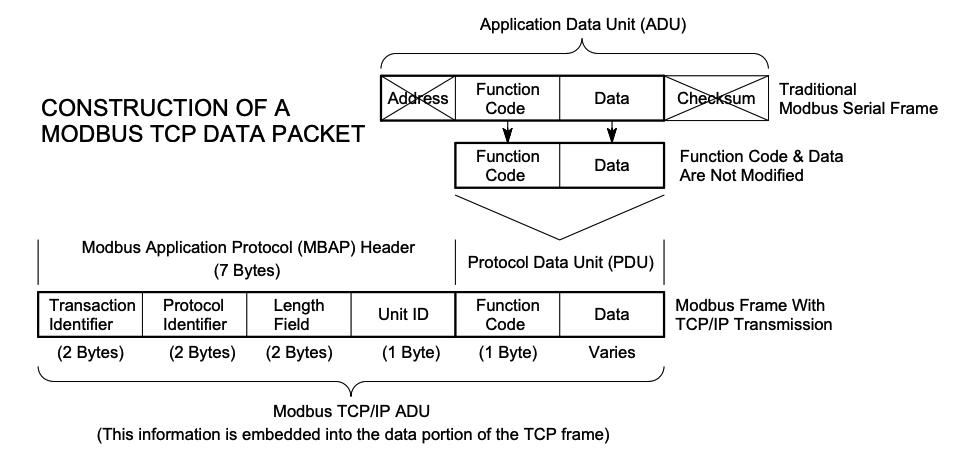
\includegraphics[width=10cm]{./graphics/Modbus-TCP-schema.png}
    \caption{Een grafische voorstelling van een Modbus TCP Data pakket. \autocite{Acromag2005}}
    \label{fig:modbus-data-pakket}
\end{figure}

\section{dataregisters}
\label{sec:stand-van-zaken-dataregisters}

Aangezien het Modbus protocol gebruikt wordt om een verbinding te kunnen maken met de nodige apparatuur, moet ook bekend zijn welke data registers gebruikt moeten worden.\\

Om de metingen van de Siemens PAC2200 op te halen, wordt data register 65 uitgelezen, in dit register staat het totaal actief vermogen opgeslagen. Dit register is nodig om te weten of er energie opgewekt of aangekocht wordt. Nadat de waarde is opgehaald wordt er nog een berekening uitgevoerd om deze waarde in de juiste eenheid weer te geven.\\

Voor de laadpaal aan te sturen zijn er meerdere registers die gebruikt kunnen worden. Hier is een lijst van de data registers die carwash Clean Car belangrijk vindt:

\begin{itemize}
    \item Modbus Slave Max Current (1210) - Dit register wordt gebruikt om de maximale stroom, die de laadpaal mag gebruiken, te bepalen.
    \item Real Energy Consumed Sum (390) - Dit register geeft weer hoeveel energie de laadpaal op dat moment gebruikt.
    \item Mode 3 state (1201) - Dit register geeft de laadmodus van de laadpaal weer.
    \item Temperature (1102) - Dit register geeft de temperatuur van de laadpaal weer.
    \item Charge using 1 or 3 phases (1215) - Met dit register kan bepaald worden of de laadpaal in single- of 3-phase moet laden.
\end{itemize}

Bij deze registers, hebben registers 1210 en 1215 read/write privileges en registers 390, 1201 en 1102 read privileges, dit betekent dat registers 1210 en 1215 ook gebruikt kunnen worden om de laadpaal aan te sturen. Registers 390, 1201 en 1102 daar in tegen kunnen enkel aangesproken worden om waarden uit te lezen.

\section{Authenticatie}
\label{sec:stand-van-zaken-authenticatie}

Er zijn verschillende manieren om een gebruiker te authenticeren in een applicatie. Zo zijn ook verschillende authenticatie providers die gebruikt kunnen worden, maar aangezien de applicatie die gebouwd wordt voor Carwash Clean Car een interne applicatie is, wordt er gebruikgemaakt van een zelf geschreven authenticatie service. Deze service zal een e-mailadres en wachtwoord verwachten van de gebruiker. Als deze correct zijn, zal de service een token terugsturen naar de applicatie. Dit token wordt dan gebruikt om de gebruiker te authenticeren in de applicatie.

\section{Backend}
\label{sec:stand-van-zaken-backend}

Omdat er verschillende apparaten moeten aangestuurd worden, kan de vraag gesteld worden of dat deze allemaal rechtstreeks via de applicatie worden aangestuurd of dat er tussen de applicatie en de apparatuur, nog een extra service uitgewerkt wordt dat deze dan aanstuurt.\\

De propere oplossing is dat er een backend met verschillende endpoints wordt opgesteld, zodat alle connecties met de apparaten makkelijk te testen vallen. De bedoeling is dan dat de applicatie de juiste waarden naar de juiste endpoints stuurt, zodat de apparaten niet rechtstreeks in contact met de applicatie komen te staan.\\

De endpoints van de backend zijn opgedeeld per apparaat. Dit wil zeggen dat alle requests voor het apparaat in kwestie naar de endpoint van het apparaat in kwestie worden doorgestuurd. In lijst \ref{list:api-endpoints} vindt u de endpoints van de api terug.

\begin{itemize}
    \item \textbf{Authenticatie:} \label{list:api-endpoints}
          \begin{itemize}
              \item GET-request
                    \begin{itemize}
                        \item /login/:email
                    \end{itemize}
          \end{itemize}
    \item \textbf{Zonnepanelen:}
          \begin{itemize}
              \item GET-request
                    \begin{itemize}
                        \item /electricity/status
                    \end{itemize}
          \end{itemize}
    \item \textbf{Laadpaal:}
          \begin{itemize}
              \item GET-request
                    \begin{itemize}
                        \item /charging-station/max-current
                        \item /charging-station/energy-consumed-sum
                        \item /charging-station/mode
                        \item /charging-station/temp
                        \item /charging-station/charge/1-3-phases
                    \end{itemize}
              \item POST-request
                    \begin{itemize}
                        \item /charging-station/update-max-current
                        \item /charging-station/charge/update-1-3-phases
                    \end{itemize}
          \end{itemize}
    \item \textbf{Beluchtingssysteem:}
          \begin{itemize}
              \item GET-request
                    \begin{itemize}
                        \item /blower/status
                    \end{itemize}
              \item POST-request
                    \begin{itemize}
                        \item /blower/update-status
                    \end{itemize}
          \end{itemize}
\end{itemize}

\section{Front end}
\label{sec:stand-van-zaken-front-end}

De front end van de applicatie is een belangrijk deel van het volledige plaatje, omdat de eindgebruiker hier het meeste interactie mee heeft. Het framework dat gebruikt zal worden is React JS, omdat dit de voorkeur was van het bedrijf.\\

Uiteindelijk maakt het niet echt uit welk front end framework er gebruikt wordt, elk framework heeft zo zijn eigen voor en nadelen.

\section{Samenvatting}
\label{sec:stand-van-zaken-samenvatting}

In de literatuurstudie zijn de belangrijkste spelers aan bod gekomen en is onderzocht geweest wat er nodig is om de applicatie voor carwash clean car te bouwen. Zo is er ook een diepere kennis opgedaan over de belangrijkste spelers, om het project met succes af te kunnen ronden. \\

Er is besproken hoe er aan de data van de zonnepanelen geraakt kon worden en hoe deze data gebruikt kan worden om bepaalde bedrijfsprocessen aan te sturen wanneer er genoeg elektriciteit opgewekt wordt met de zonnepanelen.\\

Het volgende deel van deze literatuurstudie had te maken met de laadpaal die geïnstalleerd staat aan het bedrijf. Zo is er onderzocht geweest hoe deze aangesproken kon worden.\\

Na de eerste 2 hoofdstukken is er besproken hoe het beluchtingssysteem slim bestuurd kan worden. Zo werd door het bedrijf gecommuniceerd dat deze is aangesloten op een smart plug, die verbonden is met het internet. Hierdoor kan deze ook makkelijk van op afstand aan en af gezet worden.\\

Nadien werden de gebruikte protocollen uitgebreid besproken. In dit hoofdstuk werd er eerst een kleine geschiedenis van het Modbus protocol verwoordt en werd uitgelegd hoe het Modbus TCP/IP en Modbus TCP/IP Slave protocol werkt.\\

Na dit hoofdstuk werden de data registers die nodig zijn om te weten of er elektriciteit aangekocht of opgewekt wordt besproken. Zo werden ook de registers in verband met de laadpaal die belangrijk zijn voor carwash clean car opgesomd, hier werd per register ook een klein woordje uitleg bij gegeven om te weten wat welk register juist doet.\\

Tussen het hoofdstuk van de data registers en de backend kawm het hoofdstuk over authenticatie aan bod. Hier werd besproken hoe de gebruiker geauthenticeerd wordt in de applicatie.\\

In het voorlaatste deel van de literatuurstudie werd de backend besproken. Hier werd aangetoond dat deze nodig is om de applicatie makkelijker te beheren. Er werd ook een oplijsting gemaakt van alle endpoints.\\

Als laatste werd de front end besproken, hier werd aangehaald welke front end framework gebruikt wordt in de proefopstelling.